\documentclass[mat1, tisk]{fmfdelo}
% \documentclass[fin1, tisk]{fmfdelo}
% Če pobrišete možnost tisk, bodo povezave obarvane,
% na začetku pa ne bo praznih strani po naslovu, …

%%%%%%%%%%%%%%%%%%%%%%%%%%%%%%%%%%%%%%%%%%%%%%%%%%%%%%%%%%%%%%%%%%%%%%%%%%%%%%%
% METAPODATKI
%%%%%%%%%%%%%%%%%%%%%%%%%%%%%%%%%%%%%%%%%%%%%%%%%%%%%%%%%%%%%%%%%%%%%%%%%%%%%%%

% - vaše ime
\avtor{Tjaž Eržen}

% - naslov dela v slovenščini
\naslov{Paralelizacija grafovskih algoritmov v funkcijskih programskih jezikih}

% - naslov dela v angleščini
\title{Parallelisation of Graph Algorithms in Functional Programming Languages}

% - ime mentorja/mentorice s polnim nazivom:
\mentorica{izr.~prof.~dr.~Matija Pretnar}

% - leto diplome
\letnica{2023} 



% - povzetek v slovenščini
%   V povzetku na kratko opišite vsebinske rezultate dela. Sem ne sodi razlaga
%   organizacije dela, torej v katerem razdelku je kaj, pač pa le opis vsebine.
\povzetek{TODO}

% - povzetek v angleščini
\abstract{TODO}

% - klasifikacijske oznake, ločene z vejicami
%   Oznake, ki opisujejo področje dela, so dostopne na strani https://www.ams.org/msc/
\klasifikacija{68R10, 68W10, 68N18, 68N19, 05C85}

% - ključne besede, ki nastopajo v delu, ločene s \sep
\kljucnebesede{TODO}

% - angleški prevod ključnih besed
\keywords{TODO} % angleški prevod ključnih besed


% TODO
% - angleško-slovenski slovar strokovnih izrazov
\slovar{
% TODO: Je vztrajno dober prevod ``persistent''?
\geslo{persistent data structure}{vztrajna podatkovna struktura}
% TODO: Je minljivo dober prevod ``ephemeral''?
\geslo{ephemeral data structure}{Minljiva podatkovna struktura}
\geslo{high performance computing}{Visokozmožnostno računanje}
\geslo{domains}{domene}
\geslo{parallel tasks}{vzporedne naloge}
\geslo{task collections}{zbirke opravil}
\geslo{parallel computation patterns}{vzorci vzporednega računanja}
\geslo{synchronization primitives}{sinhronizacijski mehanizmi}
\geslo{load balancing}{Izravnavanje obremenitve}
\geslo{high-level}{visokonivojski}
\geslo{code wrapper}{programski ovoj}
\geslo{adjaceny list}{seznam sosednosti}
}

% - ime datoteke z viri (vključno s končnico .bib), če uporabljate BibTeX
% \literatura{literatura.bib}


%%%%%%%%%%%%%%%%%%%%%%%%%%%%%%%%%%%%%%%%%%%%%%%%%%%%%%%%%%%%%%%%%%%%%%%%%%%%%%%
% DODATNE DEFINICIJE
%%%%%%%%%%%%%%%%%%%%%%%%%%%%%%%%%%%%%%%%%%%%%%%%%%%%%%%%%%%%%%%%%%%%%%%%%%%%%%%

% naložite dodatne pakete, ki jih potrebujete
\usepackage{algpseudocode}  % za psevdokodo
\usepackage{algorithm}      % za algoritme
\usepackage{algorithmicx}
\usepackage{hyperref}
\usepackage{listings}
\usepackage{tikz}
\usetikzlibrary{shapes,arrows}

\hypersetup{
    colorlinks=true,
    linkcolor=blue,
    filecolor=magenta,
    urlcolor=cyan,
    citecolor=red
}

% Set the font size for all listings
\lstset{basicstyle=\footnotesize\ttfamily}

\algnewcommand\algorithmicto{\textbf{to}}
\algnewcommand\algorithmicin{\textbf{in}}
\algnewcommand\algorithmicforeach{\textbf{for each}}
\algrenewtext{For}[3]{\algorithmicfor\ #1 $\gets$ #2\ \algorithmicto\ #3\ \algorithmicdo}
\algdef{S}[FOR]{ForEach}[2]{\algorithmicforeach\ #1\ \algorithmicin\ #2\ \algorithmicdo}


\floatname{algorithm}{Algoritem}
\renewcommand{\listalgorithmname}{Kazalo algoritmov}

\newcommand{\R}{\mathbb R}
\newcommand{\N}{\mathbb N}
\newcommand{\Z}{\mathbb Z}
\newcommand{\C}{\mathbb C}
\newcommand{\Q}{\mathbb Q}

\lstdefinelanguage{OCaml}{
  keywords={let,rec,if,then,else, module},
  sensitive=true,
  basicstyle=\ttfamily,
  keywordstyle=\bfseries,
  showstringspaces=false,
  morecomment=[s]{(*}{*)},
  morestring=[b]"
}

\lstset{
  language=Caml,
  frame=single,
  numbers=left,
  numberstyle=\tiny,
  stepnumber=1,
  numbersep=5pt,
  tabsize=2,
  breaklines=true,
  prebreak=\raisebox{0ex}[0ex][0ex]{\ensuremath{\hookleftarrow}},
  showtabs=false,
  showspaces=false,
  showstringspaces=false,
  basicstyle=\ttfamily\small,
  identifierstyle=\ttfamily\small,
  commentstyle=\color{gray}\ttfamily\small,
  keywordstyle=\color{blue}\ttfamily\small,
  stringstyle=\color{red}\ttfamily\small
}


%%%%%%%%%%%%%%%%%%%%%%%%%%%%%%%%%%%%%%%%%%%%%%%%%%%%%%%%%%%%%%%%%%%%%%%%%%%%%%%
% ZAČETEK VSEBINE
%%%%%%%%%%%%%%%%%%%%%%%%%%%%%%%%%%%%%%%%%%%%%%%%%%%%%%%%%%%%%%%%%%%%%%%%%%%%%%%

\begin{document}

\section{Uvod}

Grafovski algoritmi so dan danes ključni pri modeliranju širokega nabora vsakdanjih problemov: 
Igrajo pomembno vlogo pri modeliranju družbenih ter računalniških omrežjih, z njimi pa se prav tako razrešujejo problemi na področjih računalniške komunikacije ter podatkovne analitike. 
Splošno, z grafi lahko abstrahiramo kakršno koli množico odnosov med danimi entitetami, vse od računanja razdalj med mesti, pa do računanje vodnega pretoka od enega kraja do drugega.

Ker kompleksnost grafov raste nelinearno z večanjem podatkov, z njihovim računanjem ter procesiranjem pogosto trčimo ob računsko prezahtevno oviro.
Načinov za reševanje tega je več, pogosto pa je ena izmed najpogostejših ozkih grl to, da našega programa nismo napisali paralelno ter s tem izkoristili celotne kapacitete računalnika, 
temveč smo naš program poganjali zgolj na enem jedru. 
Posledično je paralelizacija tovrstnih algoritmov v zadnjih letih postala zanimiva in aplikativna raziskovalna tema. 
V svoji diplomski nalogi se bom tako ukvarjal z paralelizacijo grafovksih algoritmov.

Funkcijski programski jeziki zagotavljajo matematične abstrakcije na višjem nivoju, kot so jih to sposobni navadni imperativni programski jeziki, kot so na primer Python, C++ in Java. 
Ena izmed prednosti funkcijskih programskih jezikov je, da omogočajo deklarativno programiranje, kar jih naredi bolj paralelizabilne (več o tem v nadaljevanju). 
Tako me je zanimanje za matematične grafe, algoritme in funkcijske jezike pripeljalo v združevanje vseh teh tem hkrati: 
V svoji diplomski nalogi se bom zato osredotočil na \textit{paralelizacijo grafovskih algoritmov v funkcijskih programskih jezikih}.

\begin{definicija}
  \textbf{Deklarativni programski jezik} je vrsta programskega jezika, kjer razvijalec opišie kaj naj program stori, namesto kako naj to stori. Programi so tipično strukturirani kot nizi deklaracij, 
  ki določajo razmerja in omejitve med med različnimi entitetami znotraj problema. Nasprotno, \textbf{imperativni programski jezik} je vrsta programskega jezika, kjer programer navede zaporedje ukazov,
  ki naj jih računalnik izvrši za rešitev problema.
\end{definicija}

Vzporednost na nivoju pomnilnika je moč doseči na dva načina: 
Tako, da je pomnilnik vsem računalniškim jedrom skupen, ali pa da je pomnilnik \textit{porazdeljen}. 
V tej diplomski nalogi se bom osredotočal na sisteme s skupnim pomnilnikom. 
V tej diplomski nalogi se bom osredotočal zgolj na sisteme s skupnim pomnilnikom ter porazdeljeno procesorsko močjo.

Vse več funkcijskih programskih jezikov, kot so na primer Scala, F\# ter Haskell ima implementirane knjižnice in ogrodja za paralelizacijo grafovskih algoritmov:
\begin{itemize}
    \item knjižnica \textit{Graphalyze} v Haskellu zagotavlja vzporedne algoritme za najkrajšo pot ter iskanje krepko povezanih komponent.
    \item \textit{GraphX} v Scali ponuja implementacijo paralelnega Googlovega PageRank algoritma.
    \item \textit{Alea.cuBase} nam ponuja osnovne paralelne algoritme v jeziku F\#.
\end{itemize}

Od konca lanskega leta pa imamo nov funkcijski programski jezik, ki je postal ``multicore'' - to je OCaml, ki se med drugim poučuje na naši fakulteti v sklopu računalniško-orientiranih predmetov. 
Zato sem to priložnost izoristil, da svoje računalniške programe pišem v tem funkcijskem jeziku. 
V tej diplomski naloge se bom tako spustil v tovrstne knjižnice v funkcijskih jezikih, ki že obstajajo, 
pregledal novejše raziskave kar se tiče grafovskih algoritmov v imperativnih jezikih, to prevedel v deklarativni jezik ter vse to skupaj povezav v zaključeno celovito knjižnico v OCamlu.

\section{Kratek uvod v funkcijsko programiranje}

\subsection{Zakaj funkcijski programski jeziki}

\begin{definicija}
\textbf{Stranski učinki} so v programiranju kakršen koli odklon med čistimi matematičnimi funkcijami ter našim programom.
\end{definicija}

\begin{definicija}
  \textbf{Funkcijsko programiranje} je računalniški koncept, znotraj katerega programe pišemo komponiranjem in apliciranjem matematičnih funkcij. 
\end{definicija}

Že po definiciji je moč čutiti, da bo taka vrsta programov v splošnem bolj podobna pisanju čistih matematičnih funkcij. Posledično programiranje take vrste uporabnika preko zasnove samega jezika
spodbudi, piše programe z manj stranskimi učinki.

Programiranje take vrste uporabnika preko zasnove samega jezika spodbudi, da piše t.i. programe brez stranskih učinkov oz. jih omeji kakor se le da. 
Primer stranskega učinka bi bilo spreminjanje uporabniškega pomnilnika, ali pa branje tekstovnih datotek.

Kot rečeno, v splošnem se stranskim učinkov želimo izogniti, saj pogosto zbegajo tako razvijalca kot tudi uporabnika: 
Sorazvijalcu zmanjšajo preglednost naše kode ter privedejo do bolj pogostih napak, iz uporabniškega stališča pa se kakšen podatek v ozadju nehote spremeni, kar uporabnika pogosto zbega. 
Tiste dele kode, ki pa stranske učinke imajo, pa izoliramo v smislu da dodatno ne počnejo še drugih čistih matematičnih operacij.

% TODO: Dodaj code snippet, kjer pokažeš, zakaj stranski učinki niso zaželjeni.

Zadnjih par let funkcijski programski jeziki zaradi svojih lastnosti pridobivajo na popularnosti. 
Zaradi zasnove funkcijskih programskih jezikov so tovrstni programi tipično lepše razdeljeni v manjše kose kode, znotraj ima vsak kot kode natanko eno funkcijo, 
kar omogoči lažjo uporabo iste programske kode na več različnih problemih. 
Zaradi takih učinkov ter drugih razlik, ki ločijo funkcijske ter imperativne jezike (npr. preverjanje tipov pred izvajanjem programa) pa je naš program prav tako precej lažje testirati, razhroščevati in vzdrževati. 
Funkcijski programer se pogosto pošali, da mu program njegovo napako sporoči že preden je program sploh zagnal. 
Tako je uporabnik ``prisiljen'' pisati bolj robustne ter zanesljive programe, manj izpostavljene potencialnim napakam ter sesutjem.

Zadnja prednost, ki bi jo izpostavil, je razlika v hitrosti funkcijskih jezikov - le-ti so po eni strani precej bolj ekpresivni od nižjenivojskih imperativnih jezikov (C++, C) 
ter le malo počasnejši kar se tiče izvajanja, po drugi strani pa precej  hitrejši od visokonivojskih programskih jezikov (Python, Ruby, Java), 
s čimer imajo dobro uporabno nišo v industriji, kjer sta važna tako hitrost kot ekspresivnost jezika (npr. uporaba takih jezikov za visoko-frekvenčno trgovanje s finančnimi instrumenti).

Kot že omenjeno v uvodu, pa funkcijski jeziki prav tako omogočajo lažjo sočasnost ter paralelizabilnost programa. 
Vse to funkcijske jezike naredi primerne za t.i. \textit{visoko performančne sisteme z večnitinimi programi} (ang. high performance computing).

% TODO: Dodaj še kaj o paralelizabilnosti tukajle.

\subsection{Funkcijske podatkovne strukture}

Ko potrebujem npr. implementacijo vrste s prednostjo v Pythonu, je pogosto dovolj, da v splošnem učbeniku najdem njeno implementacijo ter to prepišem. 
Razvijalci, ki pa svojo kodo pišejo v funkcijskih programskih jezikih, pa pogosto te sreče nimajo. 
Razloga sta dva: Prvi bi bil, da funkcijski jeziki niso tako razširjeni kot imperativni, drugi pa je, da se funkcijski jeziki med sabo bolj razlikujejo kot se med sabo razlikujejo imperativni. 
Poljubno psevdokodo, napisano v imperativnem smislu, je lažje prirediti v Python, kot pa je npr. poljubno psevdokodo, napisano v funkcijskem smislu prirediti v na primer OCaml.

\begin{definicija}
V splošnem podatkovne strukture delimo na dve skupini:
\begin{itemize}
  \item Podatkovna struktura je \textbf{vztrajna}, če lahko vidimo njeno zgodovino spreminjanja. Taka podatkovna struktura hrani svoje prejšne verzije.
  \item Podatkovna struktura je \textbf{minljiva}, je podatkovna struktura, ki ne pomni svojih prejšnih verzij.
\end{itemize}
\end{definicija}

Funkcijski programski jeziki imajo zanimivo lastnost, da so vse podatkovne strukture avtomatsko \textit{vztrajne}, 
medtem ko je v imperativnih programskih jezikih vztrajne podatkovne strukture tipično težje implementirati, prav tako pa so asimptotsko počasnejše kot ``minljive'' podatkovne strukture. 
Prednost vztrajnih podatkovnih struktur očitno ta, da lahko dostopamo do svojih prejšnjih različic, prednost minljivih struktur pa je, da da so hitrejše na pram vztrajnih. 
Posledično so v splošnem podatkovne strukture v funkcijskih jezikih asimptotsko počasnejše kot pri imperativnih jezikih.

% TODO (kasneje): Podaj primer podatkovne strukture, ki se je na funkcijski način ne da učinkovito implementirati.
Še ena slabost podatkovnih struktur v funkcijskih jezikih je, da se nekaterih podatkovnih struktur preprosto ne da učinkovito implementirati na funkcijski način.

V nadaljevanju dokumenta se bom najprej posvetil vprašanju, kako graf v funkcijskih jezikih sploh predstavimo, nato pa se bom lotil algoritmov ter podatkovnih struktur na grafih.


\section{Prestavitev grafa v funkcijskih jezikih}

Če hočemo implementirati kakršen koli grafovski algoritem, je prvi korak, da graf sploh predstavimo v našem programu. V funkcijskih programskih jezikih je naše delo žal
malce oteženo, saj so, kot že rečeno, podatkovne strukture tipično nespremenljive (ang. mutable).

Zato sem se odločil da bom graf v svoji diplomski nalogi predstavil na dva načina:
\begin{itemize}
  \item Prvi je bolj podoben imperativnemu načinu, kjer graf predstavimo s spremenljivimi podatkovnimi strukturami: Vozlišča hranimo v tabeli, povezave pa v matriki sosednosti.
        Za implementacijo uporabimo OCamlove arraye implementacija je vidna na 
        \href{https://github.com/tjazerzen/parallelisation-of-graph-algorithms-in-functional-programming-languages/blob/predstavitev_grafa_z_arrayi_ter_mnozicami/playground/graph/graph.ml}{tem naslovu}
  \item Drugi način je bolj funkcijski, kjer graf predstavimo z nespremenljivimi podatkovnimi strukturami: Namesto klasične matrike sosednosti uporabim OCamlove nespremenljive
        podatkovne strukture \texttt{map}. Ta implementacija pa je vidna na
        \href{https://github.com/tjazerzen/parallelisation-of-graph-algorithms-in-functional-programming-languages/blob/master/playground/graph/graph.ml}{tem naslovu}
\end{itemize}

\subsection{Predstavitev grafa s spremenljivo matriko sosednosti} \label{sec:predstavitev_grafa_s_spremenljivo_matriko_sosednosti}

Tu sem se odločil, da bom graf predstavil s spremenljivo spremenljivimi podatkovnimi strukturami. Definiral sem tipe \texttt{node} ter \texttt{graph} na sledeč način:

\begin{lstlisting}
type 'a node = {
  created_time: float;
  id: int;
  value: 'a;
}

module IntSet = Set.Make(struct
  type t = int
  let compare = compare
end)

type 'a graph = {
  nodes: ('a node Option.t) Array.t;
  adjacency_list: IntSet.t Array.t;
  is_directed: bool;
  node_count: int;
}
\end{lstlisting}

\begin{itemize}
  \item \texttt{node} je tip, ki predstavlja vozlišče grafa. Vsako vozlišče ima svoj \texttt{id}, vrednost \texttt{value} ter čas kreacije \texttt{created\_time}.
  \item \texttt{graph} je tip, ki predstavlja graf. Graf ima tabelo vozlišč \texttt{nodes}, matriko sosednosti \texttt{adjacency\_list}, 
        logično vrednost \texttt{is\_directed}, ki pove ali je graf usmerjen ali ne, ter število vozlišč \texttt{node\_count}.
\end{itemize}

Dodatno sem definiral metode, ki nam ustvarijo prazen graf ter vanj dodajo ter odvzemajo povezave in vozlišča. Vse te operacije so implementirane tako, da spreminjajo obstoječ seznam
vozlišč ter seznam sosednosti, ne gradijo pa novih podatkovnih struktur. Kot že rečeno, je ta implementacija vidna na 
\href{https://github.com/tjazerzen/parallelisation-of-graph-algorithms-in-functional-programming-languages/blob/predstavitev_grafa_z_arrayi_ter_mnozicami/playground/graph/graph.ml}{tem naslovu}

\subsection{Predstavitev grafa z nespremenljivimi podatkovnimi strukturami} \label{sec:predstavitev_grafa_z_nespremenljivimi_podatkovnimi_strukturami}

Tu sem se implementacije grafa lotil bolj "OCaml"-ovsko - z uporabo nespremenljivih podatkovnih struktur. Namesto tipov \texttt{node} ter \texttt{graph}
sem definiral kar modula \texttt{Node} ter \texttt{Graph} ter tako poskrbel, da je uporabniku uporaba teh podatkovnih struktur čim bolj transparentna, prav tako
pa poskrbim, da metode, ki jih želim skriti, ostanejo privatne glede na modul v katerem so te metode zapisane.

To je sledeča implementacija mojih modulov (opomba: Dejanskih implementacij metod ne prilagam, saj jih lahko najdete na 
\href{https://github.com/tjazerzen/parallelisation-of-graph-algorithms-in-functional-programming-languages/blob/master/playground/graph/graph.ml}{tem naslovu}):

\begin{lstlisting}

module Node : sig
  type elt = int
  type t

  val create : elt -> t
  val value : t -> elt
  val compare : t -> t -> int
  val to_string : t -> string
end = struct
  type elt = int
  type t = { id : int; value : elt }
  ...
end

module NodeSet = Set.Make (Node)
module NodeMap = Map.Make (Node)

module Graph : sig
  type elt = int (* node values *)
  type t (* graphs *)

  val empty : directed:bool -> t
  val add_node : Node.t -> t -> t
  val remove_node : Node.t -> t -> t
  val add_edge : Node.t -> Node.t -> t -> t
  val remove_edge : Node.t -> Node.t -> t -> t
  val nodes : t -> Node.t list
  val edges : t -> (Node.t * Node.t) list
  val to_string : t -> string
  val neighbours : Node.t -> t -> Node.t list
end = struct
  type t = {
    edges : NodeSet.t NodeMap.t;
    directed : bool;
  }
  ...
end

\end{lstlisting}

\begin{itemize}
  \item \texttt{Node} je modul, ki predstavlja vozlišče grafa. Vsako vozlišče ima svoj \texttt{id}, vrednost \texttt{value}.
        Za razliko od zgornje implementacije je ta priročnejša, saj uporabnik ne operira z ID-ji vozlišč, saj so ti skriti v modulu \texttt{Node}.
        S tem zmanjšamo možnost, da bi na primer uporabnik ustvaril dve vozlišči z istim ID-jem. Kot vidimo iz funkcijskega zapisa
        \texttt{val create : elt -> t}, je za ustvarjanje vozlišča potrebna zgolj vrednost, s katero bomo to vozlišče ustvarili.
  \item \texttt{Graph} je modul, ki predstavlja graf. Namesto klasične (spremenljive) matrike sosednjosti sem tu uporabil OCamlove
        Map-e (\url{https://ocaml.org/docs/map}), ki kot vrednost hranijo vozlišča sama, kot ključe pa množico sosednjih vozlišč.
        Poleg tega sem dodal metode, ki bi si jih tipično za graf želeli: Dodajanje ter odvzem vozlišč in povezav, pridobivanje seznama vseh vozlišč ter povezav,
        prikazovanje grafa v obliki niza ter pridobivanje seznama sosednjih vozlišč.
\end{itemize}



\subsection{Primerjava implementacij grafa} \label{sec:primerjava_implementacij_grafa}

Vsaka implementacija grafa ima svoje prednosti in slabosti. V tej sekciji bom primerjal obe implementaciji grafa, ki sem ju predstavil v 
sekcijah \ref{sec:predstavitev_grafa_s_spremenljivo_matriko_sosednosti} ter \ref{sec:predstavitev_grafa_z_nespremenljivimi_podatkovnimi_strukturami}.

Med pisanjem paralelnih grafovskih algoritmov se bom posluževal predvsem implementacije grafa z nespremenljivimi podatkovnimi strukturami, saj potem ne
naletetimo na težave s sočasnim dostopom do podatkovnih struktur. V primeru, da bi se odločil za implementacijo grafa s spremenljivimi podatkovnimi strukturami, je v
primeru sočasnega dostopa do osnovne podatkovne strukture treba poskrbeti za sinhronizacijo dostopa do le-te. Tipično to storimo tako, da med spreminjanjem to podatkovno
strukturo \textit{zaklenemo} (v OCamlu imamo za to že spisan modul \texttt{Mutex}, ki nam podatkovno strukturo zaklene: \url{https://v2.ocaml.org/api/Mutex.html}),
kar pa je pogosto precej počasnejši postopek kot pa uporaba nespremenljivih podatkovnih struktur, čeprav se to mogoče ne pozna v časovni zahtevnosti algoritma, ki ga izvajamo.

Vseeno pa je zlasti za pisanje sekvenčnih algoritmov uporaba spremenljivih podatkovnih struktur marsikdaj bolj priročna, saj nam v tem primeru ni treba skrbeti za sinhronizacijo 
dostopa do podatkovnih struktur.

Vsaka izmed implementacij ima za različne operacije različno časovno zahtevnost. V spodnji tabeli sem zbral časovno zahtevnost nekaterih operacij, ki jih bomo pogosto uporabljali.
Vedeti je treba, da časovna zahtevnost vpogleda v OCamlov \texttt{Map} (ter posledično \texttt{NodeMap}) enaka $O(\log n)$, kjer je $n$ število elementov v podatkovni strukturi.
(v ozadju so množice ter Map-i implementirane kot uravnotežena binarna drevesa, zato ima vpogled v te podatkovne strukture časovno zahtevnost $O(\log n)$).

\begin{table}[h]
  \centering
  \begin{tabular}{|c|c|c|}
  \hline
  \textbf{Operacija / implementacija} & \textbf{Spremenljive p.s.} & \textbf{Nespremenljive p.s.} \\ \hline
  \textbf{Dodajanje vozlišča} & $O(\log |V|)$ & \underline{$O(1_{amort.})$} \\ \hline
  \textbf{Odvzemanje vozlišča} & $O(|V| \log |V|)$ & \underline{$O(|V|)$} \\ \hline
  \textbf{Dodajanje povezave} & \underline{$O(\log |V|)$} & $O(|V| + |E|)$ \\ \hline
  \textbf{Odvzemanje povezave} & \underline{$O(\log |V|)$} & \underline{$O(\log |V|)$} \\ \hline
  \textbf{Soseščina($u$)} & \underline{$O(deg_Gu + \log |V|)$} & \underline{$O(deg_Gu + \log |V|)$} \\ \hline
  \end{tabular}
  \caption{Primerjava časovnih kompleksnosti operacij na grafu med različnima implementacijama. Podčrtana je tista 
  implementacija, ki je za dano metodo boljša.}
  \label{tab:primerjava_casovnih_kompleksnosti_operacij_na_grafu_med_razlicnima_implementacijama}
  \end{table}


\pagebreak

\section{Paralelizacija}

\subsection{Pregled OCamlove knjižnice \textit{Domainslib}} \label{sec:pregled_domainslib}

\href{https://github.com/ocaml-multicore/domainslib}{Domainslib} je sočasna programska knjižnica za OCaml, 
ki nam omogoča paralelizacijo na nivoju procesorja.
Ponuja nam niz abstrakcij in orodij za pisanje vzporednih in sočasnih programov. 
Zgrajena je na t.i. domenah (ang. domains). To so lahke niti, vgrajene v OCaml.

S prihodom nove različice OCaml 4.12, je Domainslib postal del standardne knjižnice OCaml, z verzije 5.0.0 pa se je ta knjižnica
še precej okrepila na svojih sposobnostih ter računskih zmožnostih.

Tukaj povzamem glavne koncepte Domainsliba, ki jih bom uporabil v svoji diplomski nalogi:

\begin{enumerate}
  \item Domene (ang. domains) so niti, ki nam zagotavljajo sočasnost v OCaml-u. 
        Po svoji zasnovi so visokonivojske ter imajo nizke stroške dodatne računske obremenitve, 
        kar omogoča ustvarjanje velikega števila sočasnih nalog. Novo domeno ustvarimo z ukazom ~\texttt{Domainslib.make}.
  \item Paralelne naloge (ang. parallel tasks): Knjižnica nam ponuja preproste funkcije za ustvarjanje in upravljanje z vzporednimi nalogami.
        Naloge so delovne enote, ki se lahko izvajajo hkrati na različnih domenah.
        Ustvarijo se s funkcijo ~\texttt{Domainslib.Task.async}, na njihovo dokončanje pa se počaka z uporabo ~\texttt{Domainslib.Task.await}
  \item Zbirke opravil (ang. task collections): Knjižnica nam ponuja zbirke opravil, ki so podobne paralelnim nalogam, 
        le da lahko v njih shranimo več nalog hkrati. Zbirke opravil so lahko uporabne, kadar želimo ustvariti več nalog hkrati, 
        vendar pa ne želimo ustvariti toliko domen, kot je nalog.
  \item Vzorci vzporednega računanja (ang. parallel computation patterns), ki so pogosto uporabni pri vzporednem programiranju.
        Na primer, vzorec ~\texttt{Domainslib.Parallel.map} nam omogoča vzporedno preslikavo funkcije na seznam elementov. 
        Podobno nam vzorec ~\texttt{Domainslib.Parallel.reduce} omogoča vzporedno zmanjševanje seznama elementov, 
        z vzorcem ~\texttt{Domainslib.Parallel.stable\_sort} vzporedno uredimo seznam elementov, 
        z ukazom ~\texttt{Domainslib.Parallel.For} pa vporedno poženemo for zanko. Vse to nam precej olajša delo, če lahko večji kos računalniške naloge
        razdelimo na manjše kose, ki jih lahko izvajamo vzporedno že preko vgrajenih funkcij.
  \item Sinhronizacijski mehanizmi (ang. synchronization primitives): Knjižnica nam ponuja sinhronizacijske pritive, ki nam omogočajo sinhronizacijo med domenami.
        Na primer, sinhronizacijski mehanizem ~\texttt{Domainslib.Sync} nam omogoča sinhronizacijo med domenami, 
        sinhronizacijski primitiv ~\texttt{Domainslib.Sync\_event} pa nam omogoča sinhronizacijo med domenami preko dogodkov.
  \item Izravnavanje obremenitve (ang. load balancing): Domainslib nam ponuja orodja za izravnavanje obremenitve, 
        ki nam omogočajo, da se obremenitev med domenami porazdeli čim bolj enakomerno.
\end{enumerate}

Na splošno knjižnica Domainslib poenostavlja postopek pisanja vzporednih in sočasnih programov v OCamlu. 
Zagotavlja nam visokonivojski (ang. high-level) vmesnik za upravljanje nalog, usklajevanje sinhronizacije in izkoriščanje vzporednosti, 
kar olajša izkoriščanje celotnega potenciala večjedrnih procesorjev ter doseganje boljše zmogljivosti.

Za več informacij in uradno izvedbo knjižnice Domainslib lahko obiščete uraden repozitorij knjižnice Domainslib na
GitHub-u na naslovu \url{https://github.com/ocaml-multicore/domainslib}.


\subsection{Paralelizacija 101: Računanje Fibonaccijevih števil}

Čeprav ne gre za grafovski algoritem, se mi je zdelo poučno, da najprej predstavim osnovne koncepte paralelizacije na preprostem primeru. 
Izbral sem si paralelno računanje Fibonaccijevih števil (na naiven način, ki, kot bomo videli, terja časovno zahtevnost $O(2^n)$).

Preprosto funkcijo, ki računa Fibonaccijevo število, lahko zapišemo na zelo preprost način:

\begin{lstlisting}
  let rec fib n =
    if n < 2 then 1
    else fib (n-1) + fib (n-2)
\end{lstlisting}

\begin{figure}[htb]
  \centering
\begin{tikzpicture}[node distance=2cm]

  \node (n0) at (0,0) {$n$};
  \node (n1) at (-2,-2) {$n-1$};
  \node (n2) at (2,-2) {$n-2$};
  \node (n3) at (-4,-4) {$n-2$};
  \node (n4) at (0,-4) {$n-3$};
  \node (n5) at (4,-4) {$n-3$};
  \node (n6) at (-5.5,-6) {$n-4$};
  \node (n7) at (-3,-6) {$n-5$};
  \node (n8) at (-1,-6) {$n-4$};
  \node (n9) at (0,-6) {...};

  \draw [->] (n0) -- (n1);
  \draw [->] (n0) -- (n2);
  \draw [->] (n1) -- (n3);
  \draw [->] (n1) -- (n4);
  \draw [->] (n2) -- (n4);
  \draw [->] (n2) -- (n5);
  \draw [->] (n3) -- (n6);
  \draw [->] (n3) -- (n7);
  \draw [->] (n4) -- (n8);
  \draw [->] (n4) -- (n9);

\label{fig:fib-graph}
% TODO: caption

\end{tikzpicture}
\end{figure}


Zato se seveda vprašamo, kako bi lahko to funkcijo paralelizirali. Očiten odgovor je, da bi lahko paralelno računali $fib(n-1)$ in $fib(n-2)$ ter to počeli,
dokler ne pridemo do baze rekurzije. To lahko predstavimo z grafom, kot je prikazano na sliki \ref{fig:fib-graph}.
Problem, na katerega sem naletel ob empiričnem testiranju svojega programa, je, da je ta način paralelizacije precej neučinkovit, 
saj računamo na prevečih nitih hkrati. Število niti ki jih ustvarimo namreč narašča eksponentno z $n$.
Zato sem se v svojem programu poslužil sledeče ideje: Paraleliziraj kose kode, ki vzamejo največ časa, 
pri čemer naredi čim manj asinhronih klicev na knjižnico Domainslib.

Spet, empirično sem ugotovil, da se neparalelni program začne zatikati tam nekje pri računanju Fibonaccijevih števil večjih od 38, zato sem program spisal tako,
da števila večja od 38 računam paralelno po zgoraj opisanem postopku (na vsakem koraku ustvarim dve asinhroni nalogi), števila manjša od 38 pa računam neparalelno.

\begin{lstlisting}
module T = Domainslib.Task

let rec fib n = if n < 2 then 1 else fib (n - 1) + fib (n - 2)

let rec fib_par pool n =
  if n <= 38 then fib n
  else
    let a = T.async pool (fun _ -> fib_par pool (n - 1)) in
    let b = T.async pool (fun _ -> fib_par pool (n - 2)) in
    T.await pool a + T.await pool b
\end{lstlisting}



Za nadaljevanje bomo potrebovali (opisno) definicijo domen pri paralelnem računanju:
\begin{definicija}
  V paralelnem računanju \textbf{domena} pomeni neodvisno računsko enoto, ki lahko sočasno dela z drugimi domenami.
  Dana domena predstavlja od drugih domen ločen izvedbeni kontekst, ki lahko vzporedno izvaja navodila in izračune.
  V kontektu paralelnega računalništva se izraz \textbf{število domen} nanaša na število vzporednih izvršilnih enot, ki so 
  trenutno na voljo za izvajanje izračunov.
\end{definicija}

Ustavim se pri najpomembnejših ukazih:
\begin{itemize}
  \item Z ukazom \texttt{module T = Domainslib.Task} ustvarimo okrajšavo za Domainslib.Task, kar nam olajša pisanje kode.
  \item Funkcija \texttt{fib\_par} sprejme objekt tipa \texttt{pool} (pool je zadolžen za inicializacijo množice domen, namenjene za 
        paralelno izvajanje. Tipično je ``pool'' inicializiran s številom domen).
  \item \texttt{fib\_par} preveri, če je število, ki ga računamo, manjše ali enako 38. 
        Če je, potem izračuna Fibonaccijevo število na klasičen način (na eni niti oz. na eni domeni).
        Sicer, pa ustvari dve asinhroni nalogi, ki računata Fibonaccijevo število za $n-1$ in $n-2$. Ti nalogi se bosta izvajali vzporedno.
\end{itemize}

Ta postopek sem pognal na računalniku z 8 jedri, ter dobil naslednje rezultate v odvisnosti od zahtevanega števila domen:

\begin{figure}[h!]
  \centering
  \caption{Čas izračuna 43. Fibonaccijevega števila v odvisnosti od števila domen}
  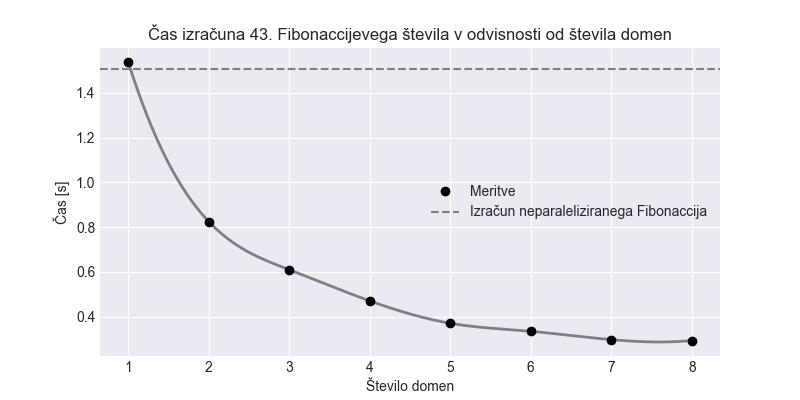
\includegraphics[width=13cm]{slike/fib_par_v_odvisnosti_od_domen.jpg}
  \label{fig:fib_par_v_odvisnosti_od_domen}
\end{figure}

Vidimo, da število domen vpliva na hitrost izračuna: Z večanjem števila domen se čas izračuna Fibonaccijevega števila zmanjšuje,
kar bi za paralelizacijo tudi pričakovali. Vendar pa se čas izračuna Fibonaccijevega števila ne zmanjšuje linearno z večanjem števila domen,
temveč sprva relativno hitro, nato pa se čas izračuna pri 14. domeni ustali tam nekje pri treh četrtinkah sekunde.
Seveda se to razlikuje od enega računalnika do drugega, razmerje med časom izračuna nekega Fibonaccijevega števila pri eni domeni ter pri
npr. desetih pa bi moralo biti podobno na vseh računalnikih (opomba: Te izračune poganjam na osemjedrnem Applovem MacBooku Air M1).

Vseeno, opomniti gre, da je točno tak eksperiment točno s takimi rezultati praktično nemogoče replicirati. Že samo s tem, da sem enkrat program poganjal
medtem ko sem imel odprte še tri druge aplikacije, drugič pa samo medtem ko sem imel odprt zgolj naš program, sem v drugem primeru dobil skoraj dvakrat hitrejši čas izračuna.

Nato pa me je še zanimalo, kako se čas izračuna Fibonaccijevih števil spreminja v odvisnosti od zahtevanega Fibonaccijevega števila ter kako se pri tem razlikuje čas izračuna
med paralelnim in neparalelnim programom. Kot že rečeno, sem empirično ugotovil, da se neparalelni program začne zatikati pri računanju Fibonaccijevih števil večjih od 38, zato
sem tako za paralelni kot neparalelni program izračunal čase izračuna Fibonaccijevih števil od 38. do vključno 45. števila. Rezultati so prikazani na 
sliki \ref{fig:fib_par_v_odvisnosti_od_n}.

\begin{figure}[h!]
  \centering
  \caption{Čas izračuna Fibonaccijevih števil v odvisnosti od zahtevanega Fibonaccijevega števila: Paralelno in neparalelno}
  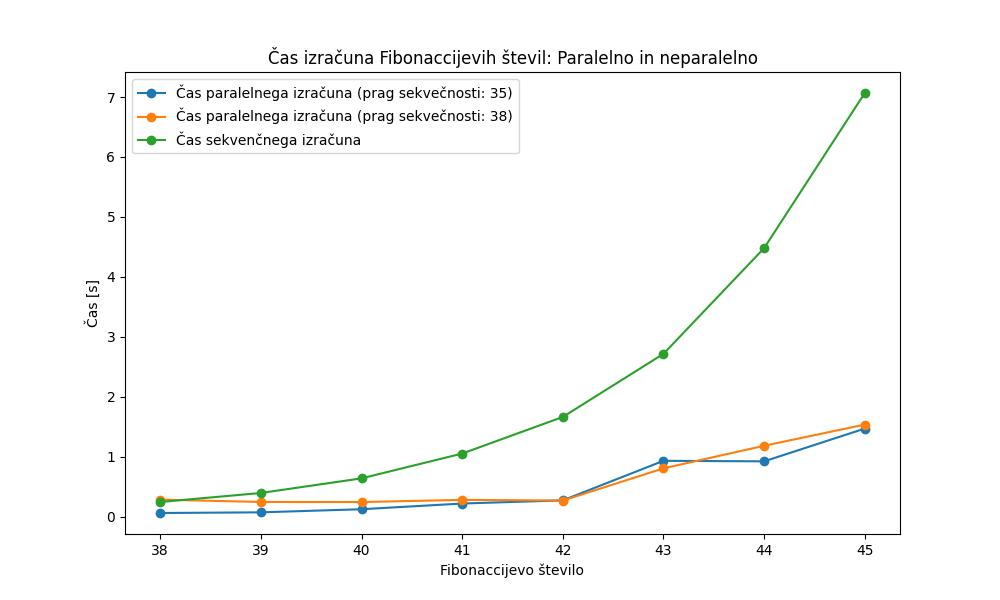
\includegraphics[width=15cm]{slike/fib_par_v_odvisnosti_od_n.jpg}
  \label{fig:fib_par_v_odvisnosti_od_n}
\end{figure}

Vidimo, da se čas izračuna Fibonaccijevih števil pri paralelnem programu z večanjem zahtevanega Fibonaccijevega števila povečuje 
počasneje kot pri neparalelnem programu. Pri neparalelnem programu se čas izvajanja, kot bi si mislili, povečuje eksponentno 
(saj je časovna zahtevnost računanja eksponentna), pri paralelnem programu pa se čas izvajanja povečuje počasneje, kar je tudi 
razvidno iz kvocienta časov izvajanja paralelnega in neparalelnega programa (označeni z svetlo modrimi kvadratki).

\section{Paralelno iskanje v širino (PBFS)}

\subsection{Neparalelni BFS}

BFS rešuje sledeč problem. Naj bo $G=(V,E)$ naš graf ter $s \in V$ naše začetno vozlišče. 
Iz danega vozlišča $s$ želimo poiskati vsa vozlišča, ki so od njega dosegljiva 
ter najti najkrajšo razdaljo od vozlišča $s$ do vseh drugih.
Drugače povedano, naš graf $G$ želimo \textit{raziskati}.

Pri predmetih iz drugega in tretjega letnika (OR, PSA1) smo se naučili, da BFS deluje tako, da
vozlišča razvršča v vrsto, nato pa iz vrste izbira vozlišča, ki jih bo raziskal.

BFS se uporablja za reševanje velikega števila problemov, kot so na primer: Raziskovanje grafa, iskanje najkrajše poti neusmerjenem v grafu,
ugotavljanje, če med dvema vozliščema obstaja pot, ugotavljanje, če je graf dvodelen, prav tako pa predstavlja osnovno za kompleksejše grafovkse
algoritme, npr. za Dijkstro.

\begin{algorithm}[H]
  \caption{Imperativno napisana psevdokoda za neparalelno iskanje v širino (BFS)}
  \label{alg:non_parallel_bfs}
  \begin{algorithmic}[1]
    \Function{BFS}{$G,s$}
      \State $Q \gets \emptyset$
      \State $Q.\text{enqueue}(s)$
      \State $visited \gets \emptyset$
      \State $visited.\text{add}(s)$
      \While{$Q \neq \emptyset$}
        \State $u \gets Q.\text{dequeue}()$
        \For{$v \in G.\text{adj}(u)$}
          \If{$v \notin visited$}
            \State $visited.\text{add}(v)$
            \State $Q.\text{enqueue}(v)$
          \EndIf
        \EndFor
      \EndWhile
    \EndFunction
  \end{algorithmic}
\end{algorithm}

Čeprav gre za neparalelen algoritem, se mi zdi še vseeno koristno predstaviti ideje algoritma, saj bomo tako lažje 
razumeli ideje kompleksnejše, paralelne verzije:
\begin{enumerate}
  \item Začni z vrsto $Q$, ki vsebuje zgolj vozlišče $s$. Odstrani vozlišče $s$ iz vrste $Q$ ter ga dodaj v množico $visited$.
        Opomniti gre, da je vrsta FIFO (first in, first out), kar pomeni, da bomo iz vrste $Q$ vedno odstranjevali vozlišča, 
        ki so bila v vrsto dodana najprej.
  \item Odstrani vozlišče $u$ iz vrste $Q$. Nato za vsako vozlišče $v$, ki je sosed vozlišča $u$ in še ni bilo obiskano,
        ga dodaj v vrsto $Q$ ter v množico $visited$. Ta postopek ponavljaj, dokler vrsta $Q$ ni prazna.
\end{enumerate}

Glavna ideja, ki je za razumevanje paralelnega postopka BFS ključna je, da vozlišča razslojimo na ekvivalenčne razrede 
glede na njihovo oddaljenost od začetnega vozlišča $s$: Razredu razdalje $0$ pripada zgolj vozlišče $s$, razredu razdalje $1$
pripadajo vozlišča, ki so od $s$ oddaljena za $1$ povezavo, in tako naprej. Dogovorimo se, da tem ekvivalenčnim razredom rečemo \textbf{nivoji}.


\subsection{Paralelni BFS}

\textbf{TODO: Priložena implementacija PBFS-ja trenutno ni funkcionalna zaradi thread safe-nessa. Ko implementacijo dokončaš, spremeni tudi spodnjo implementacijo.}

Kot že rečeno: BFS deluje z obiskovanjem vozlišč po nivojih. Glavna ideja paralelnega BFS je, da vsak nivo obiščemo vzporedno, saj so obiski vozlišč na 
istem nivoju neodvisni eden od drugega.
Na srečo ima knjižnica domainslib že implementiran programski ovoj (angl. wrapper), ki nam omogoča paralelizacijo BFS tudi na iterativen način,
kar ni tipično za funkcijski programski jezik. Tako se psevdokoda algoritma ne razlikuje veliko od neparalelne verzije, opisane v \ref{alg:non_parallel_bfs}.
Tudi če tega \textit{wrapperja} ne bi bilo spisanega, pa bi lahko paralelizacijo izvedli kar direktno preko uporabe \texttt{Domainslib.Task.async}.

\begin{lstlisting}
let bfs_parallel graph start_node num_domains =
  let queue = ref (Queue.create_empty_queue () |> Queue.enqueue start_node) in
  let visited = ref (NodeSet.empty |> NodeSet.add start_node) in
  let level = ref (NodeMap.empty |> NodeMap.add start_node 0) in

  let pool = T.setup_pool ~num_domains:(num_domains - 1) () in

  let rec bfs_inner () =
    if Queue.is_empty !queue then ()
    else
      match Queue.dequeue !queue with
      | Some (node, remaining_queue) ->
        queue := remaining_queue;
        let neighbours = Graph.neighbours node graph in
        T.parallel_for pool ~start:0
          ~finish:(List.length neighbours - 1)
          ~body:(fun i ->
            let neighbour = List.nth neighbours i in
            if not (NodeSet.mem neighbour !visited) then (
              visited := NodeSet.add neighbour !visited;
              let parent_level =
                match NodeMap.find_opt node !level with
                | Some l -> l
                | None -> failwith "Unexpected missing parent level in BFS"
              in
              level := NodeMap.add neighbour (parent_level + 1) !level;
              queue := Queue.enqueue neighbour !queue));
        bfs_inner ()
      | None -> failwith "Unexpected empty queue"
  in
  T.run pool (fun () -> bfs_inner ());
  T.teardown_pool pool;

  !level
  \end{lstlisting}

  Ker smo psevdokodo BFS-ja že opisali v \ref{alg:non_parallel_bfs}, se bom tukaj osredotočil na implementacijo samega algoritma v OCamlu:
  \begin{itemize}
    \item Najprej inicializiramo vrsto $Q$, množico $visited$ ter slovar $level$. V vrsto $Q$ dodamo začetno vozlišče $s$, v množico $visited$ dodamo $s$,
          v slovar $level$ pa dodamo par $(s, 0)$, saj je razdalja od $s$ do $s$ enaka $0$. Ti koraki so enako kot pri sekvenčnem BFS-ju.
          Ta metoda sprejme graf iz modula \texttt{Graph}, začetno vozlišče $s$ iz modula \texttt{Node} ter število domen, na katerih bomo
          naš algoritem poganjali.
    \item Nato inicializiramo domene. To naredimo z ukazom \texttt{T.setup\_pool}, ki sprejme število domen, ki jih želimo inicializirati.
          V našem primeru želimo inicializirati $n-1$ domen, kjer je $n$ število domen, ki jih ima na voljo naš procesor.
          Pozneje v kodi domene poženemo z ukazom \texttt{T.run}, nato pa jih uničimo z ukazom \texttt{T.teardown\_pool}
    \item Za pomoč pri implementaciji definiram rekurzivno metodo \texttt{bfs\_inner}. Ta metoda je ekvivalentna z zanko \texttt{while},
          ki smo jo uporabili pri neparalelni verziji BFS-ja. V tej metodi se nahaja glavna logika algoritma. Sama implementacija je precej podobna
          sekvenčni verziji - na vsakem koraku odstranimo vozlišče $u$ iz vrste $Q$, nato pa vsako vozlišče $v$, ki je sosed vozlišča $u$ in še ni bilo obiskano
          damo v vrsto ter postopek ponovimo dokler nismo obiskali vseh vozlišč v dosegu. Edina razlika je uporaba metode \texttt{T.parallel\_for}, ki paralelno 
          izvaja naše obiskovanje vozlišč.
  \end{itemize}




\end{document}